\documentclass[tikz,border=4pt]{standalone}
\usepackage{fontspec}\usepackage{xcolor}\usetikzlibrary{arrows.meta}
\setsansfont{Lato}
\begin{document}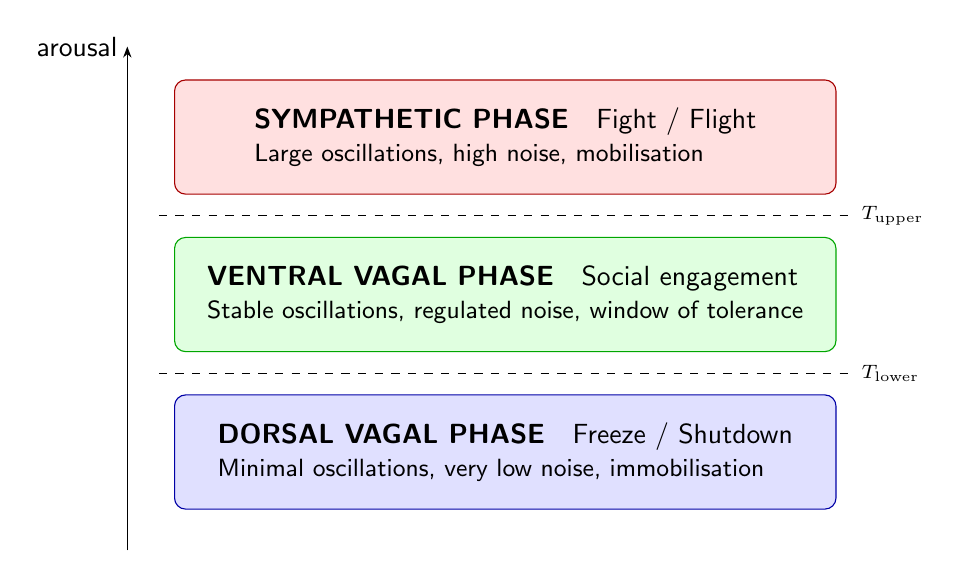
\begin{tikzpicture}[font=\sffamily,phase/.style={rounded corners=4pt,draw=#1!65!black,fill=#1!12,minimum width=8.4cm,minimum height=1.45cm,align=left,inner sep=3mm}]
\draw[-{Stealth[length=4pt]}] (0,0) -- (0,6.4) node[left]{arousal};
\node[phase=red] at (4.8,5.25) {\textbf{SYMPATHETIC PHASE}\quad Fight / Flight\\\small Large oscillations, high noise, mobilisation};
\node[phase=green] at (4.8,3.25) {\textbf{VENTRAL VAGAL PHASE}\quad Social engagement\\\small Stable oscillations, regulated noise, window of tolerance};
\node[phase=blue] at (4.8,1.25) {\textbf{DORSAL VAGAL PHASE}\quad Freeze / Shutdown\\\small Minimal oscillations, very low noise, immobilisation};
\draw[dashed] (.4,4.25) -- (9.2,4.25) node[right,font=\scriptsize] {$T_{\mathrm{upper}}$};
\draw[dashed] (.4,2.25) -- (9.2,2.25) node[right,font=\scriptsize] {$T_{\mathrm{lower}}$};
\end{tikzpicture}\end{document}
